% Options for packages loaded elsewhere
\PassOptionsToPackage{unicode}{hyperref}
\PassOptionsToPackage{hyphens}{url}
\PassOptionsToPackage{dvipsnames,svgnames,x11names}{xcolor}
%
\documentclass[
  letterpaper,
  DIV=11,
  numbers=noendperiod]{scrartcl}

\usepackage{amsmath,amssymb}
\usepackage{iftex}
\ifPDFTeX
  \usepackage[T1]{fontenc}
  \usepackage[utf8]{inputenc}
  \usepackage{textcomp} % provide euro and other symbols
\else % if luatex or xetex
  \usepackage{unicode-math}
  \defaultfontfeatures{Scale=MatchLowercase}
  \defaultfontfeatures[\rmfamily]{Ligatures=TeX,Scale=1}
\fi
\usepackage{lmodern}
\ifPDFTeX\else  
    % xetex/luatex font selection
\fi
% Use upquote if available, for straight quotes in verbatim environments
\IfFileExists{upquote.sty}{\usepackage{upquote}}{}
\IfFileExists{microtype.sty}{% use microtype if available
  \usepackage[]{microtype}
  \UseMicrotypeSet[protrusion]{basicmath} % disable protrusion for tt fonts
}{}
\makeatletter
\@ifundefined{KOMAClassName}{% if non-KOMA class
  \IfFileExists{parskip.sty}{%
    \usepackage{parskip}
  }{% else
    \setlength{\parindent}{0pt}
    \setlength{\parskip}{6pt plus 2pt minus 1pt}}
}{% if KOMA class
  \KOMAoptions{parskip=half}}
\makeatother
\usepackage{xcolor}
\usepackage[left=1in,right=1in,top=1in,bottom=1in]{geometry}
\setlength{\emergencystretch}{3em} % prevent overfull lines
\setcounter{secnumdepth}{-\maxdimen} % remove section numbering
% Make \paragraph and \subparagraph free-standing
\ifx\paragraph\undefined\else
  \let\oldparagraph\paragraph
  \renewcommand{\paragraph}[1]{\oldparagraph{#1}\mbox{}}
\fi
\ifx\subparagraph\undefined\else
  \let\oldsubparagraph\subparagraph
  \renewcommand{\subparagraph}[1]{\oldsubparagraph{#1}\mbox{}}
\fi

\usepackage{color}
\usepackage{fancyvrb}
\newcommand{\VerbBar}{|}
\newcommand{\VERB}{\Verb[commandchars=\\\{\}]}
\DefineVerbatimEnvironment{Highlighting}{Verbatim}{commandchars=\\\{\}}
% Add ',fontsize=\small' for more characters per line
\usepackage{framed}
\definecolor{shadecolor}{RGB}{241,243,245}
\newenvironment{Shaded}{\begin{snugshade}}{\end{snugshade}}
\newcommand{\AlertTok}[1]{\textcolor[rgb]{0.68,0.00,0.00}{#1}}
\newcommand{\AnnotationTok}[1]{\textcolor[rgb]{0.37,0.37,0.37}{#1}}
\newcommand{\AttributeTok}[1]{\textcolor[rgb]{0.40,0.45,0.13}{#1}}
\newcommand{\BaseNTok}[1]{\textcolor[rgb]{0.68,0.00,0.00}{#1}}
\newcommand{\BuiltInTok}[1]{\textcolor[rgb]{0.00,0.23,0.31}{#1}}
\newcommand{\CharTok}[1]{\textcolor[rgb]{0.13,0.47,0.30}{#1}}
\newcommand{\CommentTok}[1]{\textcolor[rgb]{0.37,0.37,0.37}{#1}}
\newcommand{\CommentVarTok}[1]{\textcolor[rgb]{0.37,0.37,0.37}{\textit{#1}}}
\newcommand{\ConstantTok}[1]{\textcolor[rgb]{0.56,0.35,0.01}{#1}}
\newcommand{\ControlFlowTok}[1]{\textcolor[rgb]{0.00,0.23,0.31}{#1}}
\newcommand{\DataTypeTok}[1]{\textcolor[rgb]{0.68,0.00,0.00}{#1}}
\newcommand{\DecValTok}[1]{\textcolor[rgb]{0.68,0.00,0.00}{#1}}
\newcommand{\DocumentationTok}[1]{\textcolor[rgb]{0.37,0.37,0.37}{\textit{#1}}}
\newcommand{\ErrorTok}[1]{\textcolor[rgb]{0.68,0.00,0.00}{#1}}
\newcommand{\ExtensionTok}[1]{\textcolor[rgb]{0.00,0.23,0.31}{#1}}
\newcommand{\FloatTok}[1]{\textcolor[rgb]{0.68,0.00,0.00}{#1}}
\newcommand{\FunctionTok}[1]{\textcolor[rgb]{0.28,0.35,0.67}{#1}}
\newcommand{\ImportTok}[1]{\textcolor[rgb]{0.00,0.46,0.62}{#1}}
\newcommand{\InformationTok}[1]{\textcolor[rgb]{0.37,0.37,0.37}{#1}}
\newcommand{\KeywordTok}[1]{\textcolor[rgb]{0.00,0.23,0.31}{#1}}
\newcommand{\NormalTok}[1]{\textcolor[rgb]{0.00,0.23,0.31}{#1}}
\newcommand{\OperatorTok}[1]{\textcolor[rgb]{0.37,0.37,0.37}{#1}}
\newcommand{\OtherTok}[1]{\textcolor[rgb]{0.00,0.23,0.31}{#1}}
\newcommand{\PreprocessorTok}[1]{\textcolor[rgb]{0.68,0.00,0.00}{#1}}
\newcommand{\RegionMarkerTok}[1]{\textcolor[rgb]{0.00,0.23,0.31}{#1}}
\newcommand{\SpecialCharTok}[1]{\textcolor[rgb]{0.37,0.37,0.37}{#1}}
\newcommand{\SpecialStringTok}[1]{\textcolor[rgb]{0.13,0.47,0.30}{#1}}
\newcommand{\StringTok}[1]{\textcolor[rgb]{0.13,0.47,0.30}{#1}}
\newcommand{\VariableTok}[1]{\textcolor[rgb]{0.07,0.07,0.07}{#1}}
\newcommand{\VerbatimStringTok}[1]{\textcolor[rgb]{0.13,0.47,0.30}{#1}}
\newcommand{\WarningTok}[1]{\textcolor[rgb]{0.37,0.37,0.37}{\textit{#1}}}

\providecommand{\tightlist}{%
  \setlength{\itemsep}{0pt}\setlength{\parskip}{0pt}}\usepackage{longtable,booktabs,array}
\usepackage{calc} % for calculating minipage widths
% Correct order of tables after \paragraph or \subparagraph
\usepackage{etoolbox}
\makeatletter
\patchcmd\longtable{\par}{\if@noskipsec\mbox{}\fi\par}{}{}
\makeatother
% Allow footnotes in longtable head/foot
\IfFileExists{footnotehyper.sty}{\usepackage{footnotehyper}}{\usepackage{footnote}}
\makesavenoteenv{longtable}
\usepackage{graphicx}
\makeatletter
\def\maxwidth{\ifdim\Gin@nat@width>\linewidth\linewidth\else\Gin@nat@width\fi}
\def\maxheight{\ifdim\Gin@nat@height>\textheight\textheight\else\Gin@nat@height\fi}
\makeatother
% Scale images if necessary, so that they will not overflow the page
% margins by default, and it is still possible to overwrite the defaults
% using explicit options in \includegraphics[width, height, ...]{}
\setkeys{Gin}{width=\maxwidth,height=\maxheight,keepaspectratio}
% Set default figure placement to htbp
\makeatletter
\def\fps@figure{htbp}
\makeatother

\usepackage{booktabs}
\usepackage{longtable}
\usepackage{array}
\usepackage{multirow}
\usepackage{wrapfig}
\usepackage{float}
\usepackage{colortbl}
\usepackage{pdflscape}
\usepackage{tabu}
\usepackage{threeparttable}
\usepackage{threeparttablex}
\usepackage[normalem]{ulem}
\usepackage{makecell}
\usepackage{xcolor}
\usepackage{fvextra}
\DefineVerbatimEnvironment{Highlighting}{Verbatim}{breaklines,commandchars=\\\{\}}
\DefineVerbatimEnvironment{OutputCode}{Verbatim}{breaklines,commandchars=\\\{\}}
\KOMAoption{captions}{tableheading}
\makeatletter
\makeatother
\makeatletter
\makeatother
\makeatletter
\@ifpackageloaded{caption}{}{\usepackage{caption}}
\AtBeginDocument{%
\ifdefined\contentsname
  \renewcommand*\contentsname{Table of contents}
\else
  \newcommand\contentsname{Table of contents}
\fi
\ifdefined\listfigurename
  \renewcommand*\listfigurename{List of Figures}
\else
  \newcommand\listfigurename{List of Figures}
\fi
\ifdefined\listtablename
  \renewcommand*\listtablename{List of Tables}
\else
  \newcommand\listtablename{List of Tables}
\fi
\ifdefined\figurename
  \renewcommand*\figurename{Figure}
\else
  \newcommand\figurename{Figure}
\fi
\ifdefined\tablename
  \renewcommand*\tablename{Table}
\else
  \newcommand\tablename{Table}
\fi
}
\@ifpackageloaded{float}{}{\usepackage{float}}
\floatstyle{ruled}
\@ifundefined{c@chapter}{\newfloat{codelisting}{h}{lop}}{\newfloat{codelisting}{h}{lop}[chapter]}
\floatname{codelisting}{Listing}
\newcommand*\listoflistings{\listof{codelisting}{List of Listings}}
\makeatother
\makeatletter
\@ifpackageloaded{caption}{}{\usepackage{caption}}
\@ifpackageloaded{subcaption}{}{\usepackage{subcaption}}
\makeatother
\makeatletter
\@ifpackageloaded{tcolorbox}{}{\usepackage[skins,breakable]{tcolorbox}}
\makeatother
\makeatletter
\@ifundefined{shadecolor}{\definecolor{shadecolor}{rgb}{.97, .97, .97}}
\makeatother
\makeatletter
\makeatother
\makeatletter
\makeatother
\ifLuaTeX
  \usepackage{selnolig}  % disable illegal ligatures
\fi
\IfFileExists{bookmark.sty}{\usepackage{bookmark}}{\usepackage{hyperref}}
\IfFileExists{xurl.sty}{\usepackage{xurl}}{} % add URL line breaks if available
\urlstyle{same} % disable monospaced font for URLs
\hypersetup{
  pdftitle={{[}Your Informative Title Here{]}},
  pdfauthor={Sirohi Kumar and Chaira Harder},
  colorlinks=true,
  linkcolor={blue},
  filecolor={Maroon},
  citecolor={Blue},
  urlcolor={Blue},
  pdfcreator={LaTeX via pandoc}}

\title{{[}Your Informative Title Here{]}}
\author{Sirohi Kumar and Chaira Harder}
\date{Invalid Date}

\begin{document}
\maketitle
\ifdefined\Shaded\renewenvironment{Shaded}{\begin{tcolorbox}[boxrule=0pt, interior hidden, breakable, enhanced, frame hidden, sharp corners, borderline west={3pt}{0pt}{shadecolor}]}{\end{tcolorbox}}\fi

\hypertarget{introduction}{%
\section{INTRODUCTION}\label{introduction}}

The choice of American President -- and to a lesser extent Congress --
can determine the course of public policy and politics both domestically
and internationally for the next 4 years. The election of 2000 was a
particularly controversial one in American history, especially regarding
Florida, whose close vote counts resulted in several false calls of the
election for candidate Al Gore, despite the final reports calling the
election for George Bush.

The cause of this upset can be attributed to many factors, key among
which has been identified by analysts was the unique design of the
ballot in Palm Beach County. Many Democrat voters complained the layout
of the ballot led them to accidentally choose the Reform Party Candidate
Pat Buchanan, who was projected to receive many fewer votes than he did
in Palm Beach County. In this case study, we attempt to determine if
there's evidence that Buchanan received an uncommonly high number of
votes in the 2000 election. We do so by analyzing the relationship
between the votes received by Bush (as the explanatory variable) and
Buchanan (as the response variable) across several Florida counties.

\hypertarget{results}{%
\section{RESULTS}\label{results}}

\begin{Shaded}
\begin{Highlighting}[]
\FunctionTok{library}\NormalTok{(tidyverse)}
\FunctionTok{library}\NormalTok{(Sleuth2) }
\FunctionTok{library}\NormalTok{(kableExtra)  }
\FunctionTok{library}\NormalTok{(broom)}
\FunctionTok{library}\NormalTok{(performance)}
\FunctionTok{library}\NormalTok{(ggplot2)}
\end{Highlighting}
\end{Shaded}

\hypertarget{data-wrangling}{%
\subsection{Data wrangling}\label{data-wrangling}}

The data used in this case study comes from the Sleuth2 library in R.
The dataset is of the number of votes for candidates George Bush and Pat
Buchanan in the 2000 election from each county in Florida. For our
data-wrangling process we removed one observation from the dataset. In
order to generate a model without the Palm Beach county data, we removed
the ``Palm Beach'\,' row. The dataset originally has 67 observations, so
the dataset we used for this analysis has a total of 66 observations.

\begin{Shaded}
\begin{Highlighting}[]
\CommentTok{\# Loading the case study data}
\NormalTok{election }\OtherTok{\textless{}{-}}\NormalTok{ Sleuth2}\SpecialCharTok{::}\NormalTok{ex0825}

\CommentTok{\# Creating a second dataset with Palm Beach County excluded}
\NormalTok{election\_wo\_pb }\OtherTok{\textless{}{-}}\NormalTok{ election }\SpecialCharTok{|\textgreater{}} \FunctionTok{filter}\NormalTok{(County }\SpecialCharTok{!=} \StringTok{"Palm Beach"}\NormalTok{)}
\end{Highlighting}
\end{Shaded}

\hypertarget{explore-data}{%
\subsection{Explore Data}\label{explore-data}}

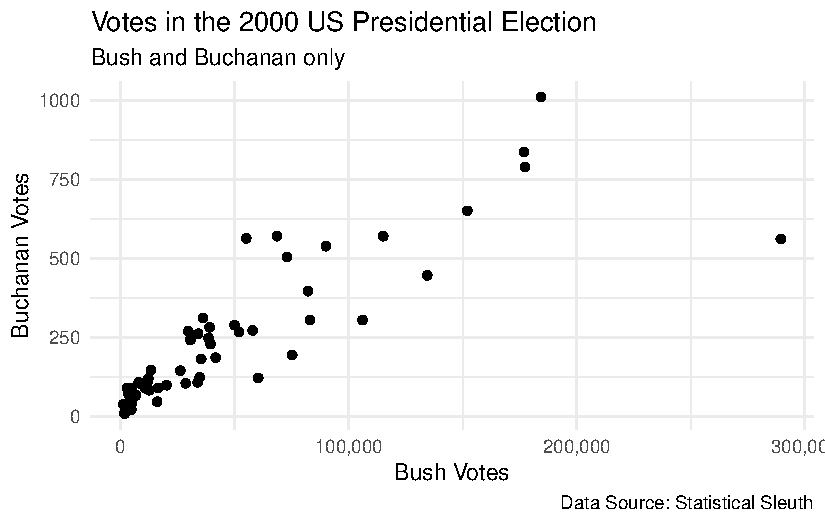
\includegraphics{sds-291_s-24_case-study-template_files/figure-pdf/unnamed-chunk-3-1.pdf}

This distribution is vaguely linear, although heavily grouped towards
the left side of the x-axis and the bottom of the y-axis. The wide range
of values on both axes, however, makes it difficult to determine the
exact relationship between these variables.

\hypertarget{find-most-appropriate-model}{%
\subsection{Find Most Appropriate
Model}\label{find-most-appropriate-model}}

\hypertarget{generate-various-models}{%
\subsubsection{Generate various models}\label{generate-various-models}}

We are generating four linear regression models to examine which would
be best suited for the prediction of Buchanan votes. The four models are
as follows:

\begin{itemize}
\tightlist
\item
  BVB: Buchanan versus Bush votes, both in original numeric value.
\item
  LVB: The natural Log of Buchanan votes versus Bush votes in original
  numeric value.
\item
  BVL: Buchanan votes in original numeric value versus the natural log
  of Bush votes.
\item
  LVL: The natural log of Buchanan versus the natural log of Bush votes.
\end{itemize}

Having each of these models will allow us to look at the statistics of
each model and decide, based on their statistics, which will fit our
prediction best.

\hypertarget{r-squared-values}{%
\subsubsection{R-Squared values}\label{r-squared-values}}

We can compare the \(R^2\) values of these various transformations using
this table, which tells us that the \texttt{ln(Buchanan)\ vs\ ln(Bush)}
model has the highest correlation of the four models.

\begin{longtable}[]{@{}
  >{\raggedleft\arraybackslash}p{(\columnwidth - 6\tabcolsep) * \real{0.2000}}
  >{\raggedleft\arraybackslash}p{(\columnwidth - 6\tabcolsep) * \real{0.2500}}
  >{\raggedleft\arraybackslash}p{(\columnwidth - 6\tabcolsep) * \real{0.2500}}
  >{\raggedleft\arraybackslash}p{(\columnwidth - 6\tabcolsep) * \real{0.3000}}@{}}
\caption{R-Squared (correlation) values for various
models}\tabularnewline
\toprule\noalign{}
\begin{minipage}[b]{\linewidth}\raggedleft
Buchanan v Bush
\end{minipage} & \begin{minipage}[b]{\linewidth}\raggedleft
ln(Buchanan) v Bush
\end{minipage} & \begin{minipage}[b]{\linewidth}\raggedleft
Buchanan v ln(Bush)
\end{minipage} & \begin{minipage}[b]{\linewidth}\raggedleft
ln(Buchanan) v ln(Bush)
\end{minipage} \\
\midrule\noalign{}
\endfirsthead
\toprule\noalign{}
\begin{minipage}[b]{\linewidth}\raggedleft
Buchanan v Bush
\end{minipage} & \begin{minipage}[b]{\linewidth}\raggedleft
ln(Buchanan) v Bush
\end{minipage} & \begin{minipage}[b]{\linewidth}\raggedleft
Buchanan v ln(Bush)
\end{minipage} & \begin{minipage}[b]{\linewidth}\raggedleft
ln(Buchanan) v ln(Bush)
\end{minipage} \\
\midrule\noalign{}
\endhead
\bottomrule\noalign{}
\endlastfoot
0.7517819 & 0.6790001 & 0.571179 & 0.8658343 \\
\end{longtable}

\hypertarget{visualize-new-model}{%
\subsubsection{Visualize new model}\label{visualize-new-model}}

\emph{describe the spread of the data in this version}

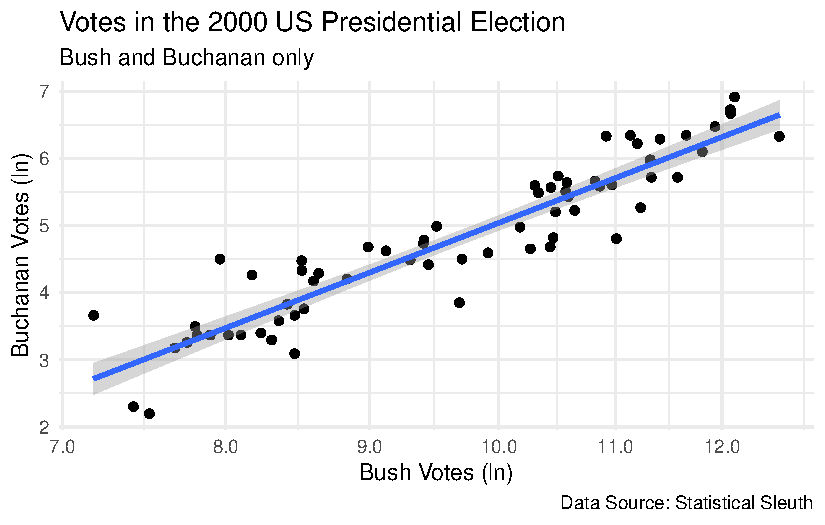
\includegraphics{sds-291_s-24_case-study-template_files/figure-pdf/unnamed-chunk-6-1.pdf}

This new visualization shows that the natural log of Bush and Buchanan's
votes have a much more linear relationship. While there's slightly more
variation towards the beginning of both axes, overall there's a high
level of correlation between the logged vote counts for both candidates,
which is reflected by the high \(R^2\) value.

\hypertarget{goodness-of-fit}{%
\subsection{Goodness of Fit}\label{goodness-of-fit}}

\hypertarget{residuals}{%
\subsubsection{Residuals}\label{residuals}}

Our selected model, in which both the Bush and Buchanan votes are
logged, yields the greatest \(R^2\) value at \(0.8658343\). With its
\(R^2\) value, it captures a stronger linear relationship than its
comparison models used (Buchanan vs Bush, \(ln(Buchanan)\) vs Bush,
Buchanan vs \(ln(Bush)\)) and also suggests a more proportional scaling
between the votes, as we can see in the visual above.

To see if our our model is truly effective and the votes in the dataset
are not random, we can use the Linearity Test, Homogeneity of Variance,
as well as the Normality of Residuals.

\hypertarget{linearity-test}{%
\paragraph{Linearity Test}\label{linearity-test}}

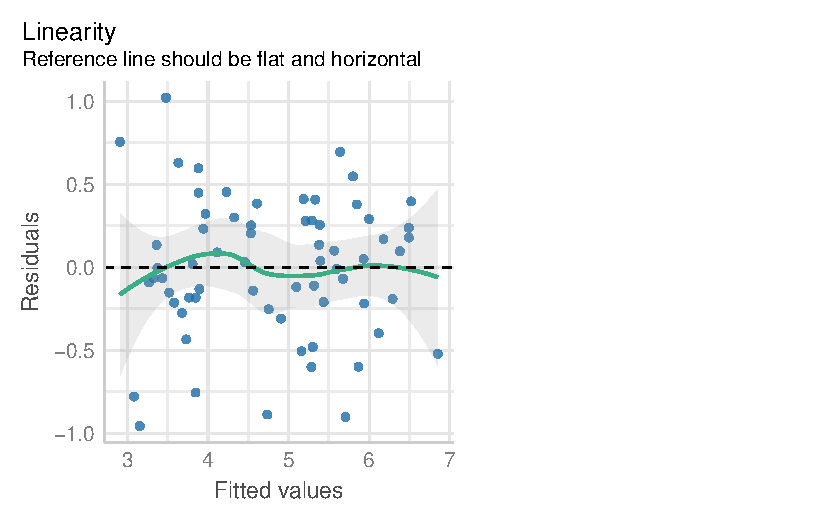
\includegraphics{sds-291_s-24_case-study-template_files/figure-pdf/unnamed-chunk-7-1.pdf}

In this case, our data do not make a flat and horizontal reference line,
thus we do not satisfy the linearity test.

\hypertarget{homogeneity-of-variance}{%
\paragraph{Homogeneity of variance}\label{homogeneity-of-variance}}

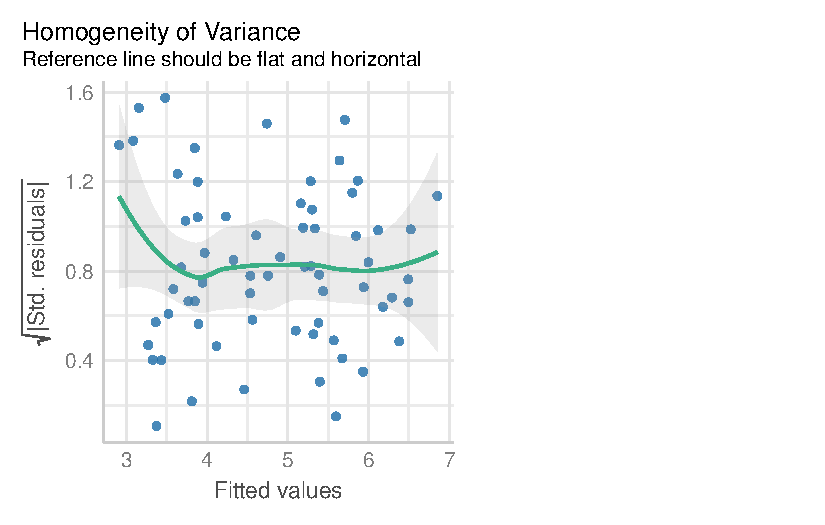
\includegraphics{sds-291_s-24_case-study-template_files/figure-pdf/unnamed-chunk-8-1.pdf}

Again, we see that our data is not linear as the variance (the points in
the plot) is scattered with no constant relationship. A linear
relationship requires constant variance.

\hypertarget{normality-of-residuals}{%
\paragraph{Normality of Residuals}\label{normality-of-residuals}}

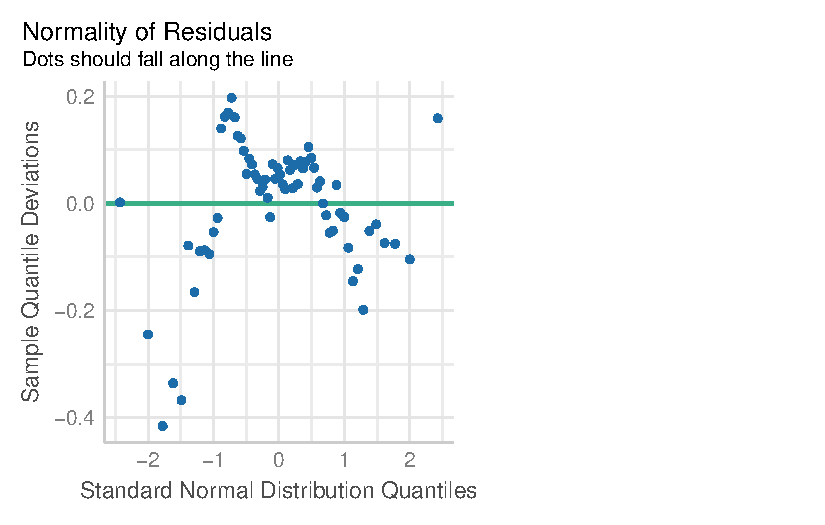
\includegraphics{sds-291_s-24_case-study-template_files/figure-pdf/unnamed-chunk-9-1.pdf}

We see in the Normality of Residuals plot above that the data points for
the sample quantile deviations vs the normal distribution quantiles do
not make a horizontal line shape.

Sources: -
http://www.sthda.com/english/articles/39-regression-model-diagnostics/161-linear-regression-assumptions-and-diagnostics-in-r-essentials/
- https://cran.r-project.org/web/packages/performance/index.html

\hypertarget{predictions}{%
\subsection{Predictions}\label{predictions}}

\hypertarget{regression-line}{%
\subsubsection{Regression Line}\label{regression-line}}

Let \(Bush_i\) denote the \(ln\) number of Bush votes in any Florida
county during the 2000 election. Using the regression model from above,
we can predict \(Buchanan_i\), the \(ln\) of the number of Buchanan
votes in any Florida county \(i\) (during the 2000 election) based on
any \(Bush_i\) value. Using this regression model, we can find
\[Buchanan_i = \beta_0 + \beta_1\left(Bush_i\right).\]

\begin{table}[H]
\centering
\begin{tabular}[t]{lcccc}
\toprule
  & Estimate & Std. Error & t value & p value\\
\midrule
(Intercept) & -2.3415 & 0.3544 & -6.6066 & 0\\
log(Bush2000) & 0.7310 & 0.0360 & 20.3229 & 0\\
\bottomrule
\end{tabular}
\end{table}

This linear model predicts that for each increase in \(ln(Bush_i)\),
that \(ln(Buchanan_i)\) should increase by \(0.7310\) votes. We can now
use this model to predict the number of votes Buchanan should have
received in Palm Beach County, if Palm Beach county was the same as the
other Florida counties.

\hypertarget{prediction-interval}{%
\subsubsection{Prediction Interval}\label{prediction-interval}}

\textbf{Obtain a 95\% prediction interval for the number of Buchanan
votes in Palm Beach from this result---assuming the relationship is the
same in this county as in the others}

\begin{table}[H]
\centering
\begin{tabular}[t]{ccc}
\toprule
center & lower & upper\\
\midrule
6.384143 & 5.524656 & 7.24363\\
\bottomrule
\end{tabular}
\end{table}

We can transform these numbers to determine the non-\(ln\) vote count.

lower: \(e^{5.524656} = 250.8\) upper: \(e^{7.24363} = 1399.164\)

Our prediction interval tells us that, based on this sample, 95\% of the
time, the number of votes for Buchanan in the 2000 election should be
between 250.8 and 1399.164 votes, given that 152,846 people voted for
Bush.

However, in the 2000 election, Buchanan received 3407 votes, which is
over twice as large as the upper bound of our interval. \emph{This
indicates that Palm Beach county's votes for Buchanan, based on Bush's
votes, are highly irregular compared to other Florida counties.}

\hypertarget{gores-votes}{%
\subsection{Gore's Votes}\label{gores-votes}}

\textbf{Assuming that some of the votes cast for Buchanan were intended
as votes for Gore, use the prediction interval to give an estimate for
the likely number of votes intended for Gore but cast for Buchanan.}

There were 3407 votes for Buchanan in the 2000 election, but our
prediction interval tells us that the number of votes expected for
Buchanan 95\% of the time is between 250.800 and 1399.164, so the likely
number of votes intended for Gore but cast for Buchanan should be
between \(3407-250.800 = 3156.200\) and \(3407-1399.164 = 2007.836\).

\hypertarget{discussion}{%
\section{DISCUSSION}\label{discussion}}

Our goal with this case study was to determine if, based on the vote
counts for Pat Buchanan and George Bush in every Florida county, we
could conclude whether Buchanan received an unusual number of votes in
Palm Beach county. We used a linear model on data that had been
transformed to show that for every increase in \(ln(Bush_i)\) by one
\(ln(Buchanan_i)\) should increase by about \(0.7310\) votes.

We used this model to generate a prediction interval that predicted with
95\% confidence that Buchanan's vote count in Palm Beach County should
have been between \(250.8\) and \(1399.164\). Instead, Buchanan received
\(3407\) votes, a highly irregular value, according to this model. Based
on this, we can conclude that there is evidence Buchanan received an
unusually high number of votes in Palm Beach county.

This deviation from the number of expected votes lends credence to the
complaints of many Democratic voters who reported having accidentally
voted for Buchanan (the Reform candidate) instead of Al Gore (the
Democratic candidate), because of the confusing ballot layout. On a
larger scale, this shows that the incredibly close election of George
Bush in 2000 may have been -- at least in part -- due to a fluke in
ballot design.

However, we can't make a conclusive claim that this is the case. First
of all, our model only calculates the correlation between Buchanan and
Bush's votes -- it cannot determine if there's a causal relationship
between the two, or indeed the existence of any causal factors affecting
the relationship between the two. Additionally, we cannot directly
attribute the unusual number of votes for Buchanan to the ballot layout,
as we haven't examined any other elections with strange ballots and,
again, this is not a causal model.

\begin{center}\rule{0.5\linewidth}{0.5pt}\end{center}

\hypertarget{r-appendix}{%
\section{R APPENDIX}\label{r-appendix}}

\emph{Copy and paste all code that you used for your case study into one
chunk at the end of your written report. Before submitting your case
study, take one final look at the R Appendix and make sure that all code
is clearly visible. If you see a line running off the side of the PDF,
please split the code over multiple lines using a linebreak.}

\begin{Shaded}
\begin{Highlighting}[]
\CommentTok{\# importing our necessary libraries}
\FunctionTok{library}\NormalTok{(tidyverse)}
\CommentTok{\# Sleuth2 contains the data used in this analysis}
\FunctionTok{library}\NormalTok{(Sleuth2) }
\CommentTok{\# to make tables in R}
\FunctionTok{library}\NormalTok{(kableExtra) }
\CommentTok{\# for data wrangling}
\FunctionTok{library}\NormalTok{(broom)}
\CommentTok{\# for residual testing}
\FunctionTok{library}\NormalTok{(performance)}
\CommentTok{\# for our plot visualizations}
\FunctionTok{library}\NormalTok{(ggplot2)}

\CommentTok{\# {-}{-}{-}{-}{-}{-}{-}{-}{-}{-}{-}{-}{-}{-}}

\CommentTok{\# Loading the case study data}
\NormalTok{election }\OtherTok{\textless{}{-}}\NormalTok{ Sleuth2}\SpecialCharTok{::}\NormalTok{ex0825}

\CommentTok{\# data wrangling:}
\CommentTok{\# Creating a second dataset EXCLUDING Palm Beach County }
\NormalTok{election\_wo\_pb }\OtherTok{\textless{}{-}}\NormalTok{ election }\SpecialCharTok{|\textgreater{}} \FunctionTok{filter}\NormalTok{(County }\SpecialCharTok{!=} \StringTok{"Palm Beach"}\NormalTok{)}

\CommentTok{\# data exploration and visualization: }
\CommentTok{\# visualizing our initial data using a scatterplot}
\FunctionTok{ggplot}\NormalTok{(}\AttributeTok{data =}\NormalTok{ election\_wo\_pb, }\FunctionTok{aes}\NormalTok{(}\AttributeTok{x =}\NormalTok{ Bush2000, }\AttributeTok{y =}\NormalTok{ Buchanan2000)) }\SpecialCharTok{+}
  \FunctionTok{geom\_point}\NormalTok{() }\SpecialCharTok{+}
  \FunctionTok{scale\_x\_continuous}\NormalTok{(}\AttributeTok{labels =}\NormalTok{ scales}\SpecialCharTok{::}\NormalTok{comma) }\SpecialCharTok{+} 
  \FunctionTok{xlab}\NormalTok{(}\StringTok{"Bush Votes"}\NormalTok{) }\SpecialCharTok{+}
  \FunctionTok{ylab}\NormalTok{(}\StringTok{"Buchanan Votes"}\NormalTok{) }\SpecialCharTok{+} 
  \FunctionTok{labs}\NormalTok{(}\AttributeTok{title =} \StringTok{"Votes in the 2000 US Presidential Election"}\NormalTok{, }\AttributeTok{subtitle =} \StringTok{"Bush and Buchanan only"}\NormalTok{, }\AttributeTok{caption =} \StringTok{"Data Source: Statistical Sleuth"}\NormalTok{) }\SpecialCharTok{+}
  \FunctionTok{theme\_minimal}\NormalTok{()}
\end{Highlighting}
\end{Shaded}

\begin{figure}[H]

{\centering 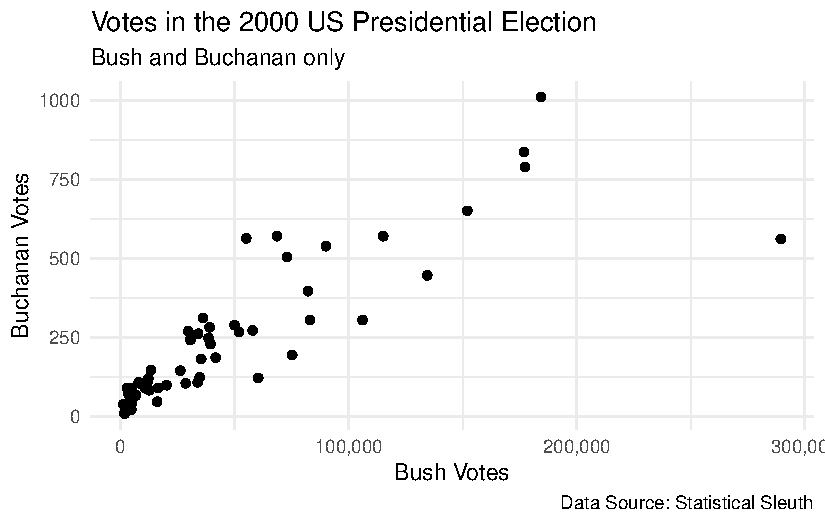
\includegraphics{sds-291_s-24_case-study-template_files/figure-pdf/unnamed-chunk-12-1.pdf}

}

\end{figure}

\begin{Shaded}
\begin{Highlighting}[]
\DocumentationTok{\#\# Bush vs Buchanan}
\NormalTok{model\_bvb }\OtherTok{\textless{}{-}} \FunctionTok{lm}\NormalTok{(Buchanan2000 }\SpecialCharTok{\textasciitilde{}}\NormalTok{ Bush2000, }\AttributeTok{data =}\NormalTok{ election\_wo\_pb)}
\NormalTok{BVB }\OtherTok{\textless{}{-}} \FunctionTok{summary}\NormalTok{(model\_bvb)}\SpecialCharTok{$}\NormalTok{r.squared}

\DocumentationTok{\#\# log(Bush) vs Buchanan}
\NormalTok{model\_lvb }\OtherTok{\textless{}{-}} \FunctionTok{lm}\NormalTok{(Buchanan2000 }\SpecialCharTok{\textasciitilde{}} \FunctionTok{log}\NormalTok{(Bush2000), }\AttributeTok{data =}\NormalTok{ election\_wo\_pb)}
\NormalTok{LVB }\OtherTok{\textless{}{-}} \FunctionTok{summary}\NormalTok{(model\_lvb)}\SpecialCharTok{$}\NormalTok{r.squared}

\DocumentationTok{\#\# Bush vs log(Buchanan)}
\NormalTok{model\_bvl }\OtherTok{\textless{}{-}} \FunctionTok{lm}\NormalTok{(}\FunctionTok{log}\NormalTok{(Buchanan2000) }\SpecialCharTok{\textasciitilde{}}\NormalTok{ Bush2000, }\AttributeTok{data =}\NormalTok{ election\_wo\_pb)}
\NormalTok{BVL }\OtherTok{\textless{}{-}} \FunctionTok{summary}\NormalTok{(model\_bvl)}\SpecialCharTok{$}\NormalTok{r.squared}

\DocumentationTok{\#\# log(Bush) vs log(Buchanan)}
\NormalTok{model\_lvl }\OtherTok{\textless{}{-}} \FunctionTok{lm}\NormalTok{(}\FunctionTok{log}\NormalTok{(Buchanan2000) }\SpecialCharTok{\textasciitilde{}} \FunctionTok{log}\NormalTok{(Bush2000), }\AttributeTok{data =}\NormalTok{ election\_wo\_pb)}
\NormalTok{LVL }\OtherTok{\textless{}{-}} \FunctionTok{summary}\NormalTok{(model\_lvl)}\SpecialCharTok{$}\NormalTok{r.squared}
\end{Highlighting}
\end{Shaded}




\end{document}
